\chapter{Analýza a klasifikácia cytometrických dát}
\label{DeepCyTOF_kap3}

Cytometrické dáta poskytujú informácie o bunkových vlastnostiach a ich správaní. Cytometria je vedná disciplína, ktorá skúma bunkové dáta a na základe nadobudnutých informácií produkuje patogenézu. Patogenáza opisuje zmeny bunkových vlastností v závislosti od rôznych chorôb. Cytometria sa využíva v biomedicíne a pri lekárskej diagnostike. Využitím cytometrie je môžné skúmať vlastnosti chorých a zdravých buniek a pozorovať, ako sa tieto vlastnosti menia v závislosti od rôznych ochorení. Vďaka týmto pozorovaniam je v dnešnej dobe možné predpokladať výskyt rôznych chorôb a diagnostikovať ich v ranných štádiách. 

V praxi sa používajú rôzne metódy na analýzu cytometrických dát. Od roku 1968 bola najčastejšie používaná metóda prietokovej cytometrie (FCM, z angl. Flow Cytometry). Táto metóda skúma krvné bunky z krvných vzoriek ktoré boli získané štandardným odberom krvy \cite{Li2016}. Metóda je založená na báze fluorescencie, skúmania buniek v pohybe \cite{Roubalova1934}. Moderná prietoková cytometria pozoruje 15-20 parametrov pre každú bunku z krvnej vzorky \cite{Roubalova1934}. Skúmaním týchto parametrov na veľmi veľkej množine rôznych vzoriek je možné vytvárať patogenézu širokého spektra ľudských ochorení \cite{Li2017}. 

Novšia metóda skúmania buniek je hmotnostná cytometria. Hmotnostná cytometria (z angl. Cytometry by Time-Of-Flight, CyTOF) je moderný spôsob analýzy cytometrických dát pri ktorom sa skúmanie zameriava na veľké množstvo vlastností jednej konkrétnej bunky. Hmotnostná cytometria je založená na pozorovaní doby preletu s využitím izotopov tažkých kovov \cite{Roubalova1934}. Moderné prístroje hmotnostnej cytometrie sú schopné pozorovať viac ako 40 bunkových parametrov \cite{Roubalova1934, Li2017}. Vďaka týmto technológiam sa ponúka možnosť detailného profilovania rôznych buniek. V praxi je metóda profilovania buniek využívaná na charakterizovanie krvných buniek, NK buniek (NK, z angl. Natural Killer), kožných buniek, celiatických buniek, reagujúcich fenotypov rakoviny atď. Charakterizovanie týchto jednotlivých typov buniek pomocou FCM alebo CyTOF umožňuje pochopenie správania jednotlivých buniek v procese choroby \cite{Li2016}.

Jeden z najdôležitejších krokov pri analýze cytometrických dát pomocou metód FCM a CyTOF je gating. Gating predstavuje zaraďovanie jednotlivých buniek do diskrétnej skupiny bunkových typov. Tento proces vyžaduje vytváranie polygónov medzi jednotlivými markermi skúmaných krvných vzoriek. Krvné markery predstavujú špecifické látky, resp. protilátky, obsiahnuté v krvy, ktorých zvýšená hodnota implikuje prítomnosť choroby. Čas potrebný na realizáciu cytometrickej analýzy je závislý na počte krvných vzoriek a na počte skúmaných markerov. Vytváranie polygónov vyžaduje porovnávanie všetkých markerov navzájom a čas potrebný na realizáciu analýzy je kvadratický vzhľadom na počet markerov \cite{Li2016}. 

Vzhľadom na náročnosť a zdĺhavosť manuálnej cytometrickej analýzy bolo žiadúce celý tento proces automatizovať. Najnovšie metódy na analýzu cytometrických dát zahŕňajú prístup strojového učenia \cite{Li2016}. Tieto metódy sa pokúšajú proces analýzy automatizovať a zvyšovať jeho škálovateľnosť a výkonnosť. Hoci sú tieto prístupy schopné automatizovať gatovanie, v konečnom dôsledku nie sú vhodné na bežné použitie kde analýza musí byť štandardizovaná, repordukovateľná, interpretovateľná a porovnateľná. Doposiaľ žiadna metóda, ktorá sa zameriavala automatickým gatingom, nebola z formálneho hľadiska akceptovaná ako zlatý štandard ktorý by mohol nahradiť manuálny gating \cite{Li2017}.

Odstupom času, hlboké neurónové učenie začalo dosahovať vynikajúce výsledky v rôznych výpočtových úlohách. Podľa zdroja \cite{Li2016}, je možné tento prístup aplikovať aj na tak komplexnú problematiku akou je cytometrická analýza. V prípade cytometrickej analýzy je počet skúmaných inštancií (krvných buniek) niekoľkonásobne vyšší ako počet skúmaných parametrov (markerov). Ak disponujeme veľkým množstvom dát (krvných buniek) ktoré obsahujú špeciálne parametre (markery), ktoré je možné využiť na klasifikáciu daných buniek, tak je možné trénovať klasifikátor ktorý bude schopný automaticky zaraďovať jednotlivé krvné bunky do diskrétnych bunkových skupín \cite{Li2016}.

Cieľom automatického gatingu je automatizovať klasifikáciu buniek bez ohľadu na pôvod meracieho prístroja, ktorý meria parametre jednotlivých buniek. Ukázalo sa, že v praxi vzniká problém takzvaného \textit{dávkového efektu}. Tento problém je zapríčinený rôznou kalibráciou meracích prístrojov. Keďže jednotlivé meracie prístroje môžu mať nastavenú inú kalibráciu, tak aj výsledky meraní, ktoré boli realizované na týchto prístrojoch, nadobúdajú inú distribúciu hodnôt. Distribúcia hodnôt parametrov buniek má signifikantný vplyv na klasifikátor \cite{Li2017}.

Na zjednotenie distribúcií hodnôt bunkových parametrov sa využíva metóda \textit{doménovej adaptácie}. \textit{Doménová adaptácia} predstavuje metódu optimalizácie distribúcie hodnôt parametrov jednotlivých inštancií. Táto metóda transformuje distribúciu hodnôt cieľovej vzorky na distribúciu hodnôt zdrojovej vzorky. Výsledná transformovaná distribúcia cieľovej vzorky je príbuzná distribúcii zdrojovej vzorky ale nie je ekvivalentná. \textit{Doménová adaptácia} slúži na minimalizáciu generalizačnej chyby inštancií cieľovej domény. Využitím doménovej adaptácie je klasifikačný model (v tomto prípade neurónová sieť) schopný klasifikovať dáta merané na rôznych prístrojoch \cite{Li2016, Li2017}.

V dávkových sadách okrem \textit{dávkového efektu} vzniká aj problém chýbajúcich hodnôt parametrov jednotlivých buniek. Pre dosiahnutie čo najkvalitnejších výsledkov je nevyhnutné nahradiť chýbajúce hodnoty z dátovej sady reálnymi hodnotami. 

Zdroj \cite{Li2017} uviedol metódu zvanú DeepCyTOF, ktorá integruje mechanizmus na elimináciu chýbajúcich hodnôt, mechanizmus na minimalizáciu generalizačnej chyby (dávkového efektu) a klasifikátor ktorý automatizuje gating jednotlivých buniek. Nahradenie chýbajúcich hodnôt je realizované takzvaným odšumujúcim autoenkóderom, DAE (z angl. Denoising AutoEncoder). Po nahradení chýbajúcich hodnôt je vykonaná kalibrácia hodnôt všetkých parametrov (doménová adaptácia). Metóda DeepCyTOF v rámci doménovej adaptácie vyžaduje jednu manuálne gatovanú dátovú vzorku (referenčnú vzorku) podľa ktorej prispôsobí všetky ostatné vzorky z dátovej sady. Doménovej adaptácií predchádza logaritmická transformácia a štandardizácia parametrov buniek \cite{Li2017}. 

Kalibrácia parametrov je realizovaná prostredníctvom špeciálnej reziduálnej siete zvanej MMD-ResNet (z angl. Maximum Mean Discrepancy Residual Network). MMD-ResNet kalibruje číselné hodnoty parametrov z cieľovej vzorky na základe parametrov referenčnej vzorky \cite{Li2016}. Samotný automatický gating je vykonávaný v poslednej fáze metódy, jednoduchou doprednou neurónovou sieťou \cite{Li2017}.

V ďalších častiach tejto kapitoly si priblížime architektúru metódy DeepCyTOF a pozrieme sa na to, ako jednotlivé komponenty matódy participujú na automatizácii procesu gatovania. Pokračovanie tejto kapitoly sa bude venovať jednotlivým transformáciám a modifikáciám dátovej sady pred finálnym gatovaním. Zameriame sa na komponenty metódy DeepCyTOF a podrobne priblížime reziduálnu sieť využívajúcu funkciu maximálnej priemernej odchýlky.

\begin{comment}
\section{Dátové sady cytometrických dát}

\subsection{Dátová sada FlowCAP-I}

Dátová sada FlowCAP-I obsahuje informácie o imunitných bunkách nachádzajúcich sa v ľudskej krvi. Tieto informácie boli získané prietokovou cytometriou. Zdroj \cite{Li2016} uviedol, že pri svojom experimente s metódou DeepCyTOF kategorizoval bunky týchto typov:
\begin{enumerate}
    \item \textit{Veľké difúzne B-bunkové lymfómy}, DLBCL (z angl. Diffused large B-cell lymphoma)
    \item \textit{Symptomatický vírus západného nílu}, WNL (z angl. West Nile Virus)
    \item \textit{Bežný darca}, ND (z angl. Normal Donors)
    \item \textit{Transplantované krvotvorné kmeňové bunky}, HSCT (z angl. Hematopoietic Stem Cell Transplant)
    \item \textit{Bunky choroby štepu-proti-hostiteľovi}, GVHD (z angl. Graft-Versus-Host Disease)
\end{enumerate}
Dátova sada disponuje výsledkami gatovania ktoré bolo vykonané manuálnym spôsobom expertnou analýzou \cite{Li2017}. Vďaka týmto výsledkom je možné vyhodnotiť úspešnosť automatického gatovania.

\subsection{Dátová sada hmotnostnej cytometrie}

Rovnako ako aj prvá dátová sada, tak aj táto obsahuje imunitné bunky získané z ľudskej krvy. Táto dátová sada pozostáva z jednotlivých súborov ktoré obsahujú cytometrické dáta rôznych subjektov:
\begin{enumerate}
    \item 14 subjektov (8 asymptomatických a 6 závažných) s historickými informáciami o infekcii vírusom západného Nílu, WNV (z angl. West Nile Virus).
    \item 34 zdravých subjektov rôzneho veku (20 mladých a 14 starých). 
\end{enumerate}
Všetky tieto krvné vzorky z týchto súborov obsahujú informáciu o hodnote 42 markerov. Z týchto 42 markerov je však pre výslednú klasifikáciu relevantných len 12. Vybrané markery sú: HLA-DR, CD4, CD8, CD3-UCH1, CD16, CD33, CD19, CD14, CD56, DNA1, DNA2 a cisplatina \cite{Li2017}. Na základe hodnôt jednotlivých markerov je možné klasifikovať jednotlivé bunky do jednej zo šiestich katogórií - 
\begin{enumerate*}
    \item B bunky,
    \item CD4+ T bunky,
    \item CD8+ T bunky,
    \item Monocyty,
    \item NK bunka,
    \item nezaradené,
\end{enumerate*}
Všetky vzorky v tejto dátovej sade boli manuálne gatované a vďaka tomu je možné vyhodnotiť presnosť predikcií neurónovej siete ktorá predikuje kategórie pre jednotlivé vzorky \cite{Li2017}.
\end{comment}

\section{Metóda DeepCyTOF}

Pred aplikovaním metódy DeepCytof na dátovú sadu, je potrebné vykonať predspracovanie hodnôt parametrov. V rámci predspracovania sú všetky dáta upravené logaritmuckou transformáciou
\begin{equation}
    A_{i,j} = log(1+A_{i,j}),
\end{equation}
kde $A_{i,j}$ predstavuje hodnotu parametra krvnej vzorky $A$. Následne je vykonaná štandardizácia všetkých parametrov krvnej vzorky $A$. Po dokončení prvotnej prípravy, je nevyhnutné nahradiť chýbajúce hodnoty a kalibrovať cieľové vzorky voči referenčnej vzorke. Po vykonaní potrebných modifikácií je možné vykonať samotné gatovanie \cite{Li2017}. 

Metóda DeepCyTOF je zložená z troch neurónových sieti. Prvá neurónová sieť, DAE, nahrádza chýbajúce dáta reálnymi číslami. Druhá neurónová sieť, MMD-ResNet, kalibruje cieľové vzorky voči referenčnej vzorke. Tretia neurónová sieť, hĺboká dopredná neurónová sieť, vykonáva finálnu klasifikáciu (gating) buniek do diskrétnych bunkových skupín \cite{Li2017}. 

Zdroj \cite{Li2017} vykonal experiment s využitím metódy DeepCyTOF, v ktorom sa snažil preukázať vplyv kalibrácie a odšumenia na kvalitu predikcie. V tomto experimente vykonával automatický gating bez použitia DAE a následne aj bez použitia MMD-ResNet. Vzhľadom k tomu, že výsledné predikcie boli porovnateľne menej kvalitné ako v prípade použitia DAE a MMD-ResNet, tak v ďalších častiach sa týmto alternatívam venovať nebudeme.

\subsection{Nahradenie chýbajúcich hodnôt odšumujúcim autoenkóderom}

Cytometrické dátové sady obsahujú množstvo nulových hodnôt. Tieto nulové hodnoty je možné interpretovať ako chýbajúce hodnoty. Nulové hodnoty sú spôsobené nestabilitou meracieho prístroja a v skutočnosti nereprezentujú pravú hodnotu 0 \cite{Li2017}.

Nahradenie nulových hodnôt za reálne hodnoty je realizované odšumujúcim autoenkóderom, DAE (z angl. Denoising AutoEncoder). DAE je druh malej neurónovej siete, ktorá je trénovaná na rekonštrukciu "vyčisteného vstupu" na základe jeho poškodenej verzie. Pozostáva zo skrytých vrstiev ktoré disponujú ReLU na každej vrstve \cite{Li2017}.

DAE je trénovaný na dátovej sade buniek, bez nulových hodnôt (alebo s veľmi nízkym výskytom). Pre zvýšenie kvality predikcie, je vytvorená simulácia nestability meracieho prístroja, ktorá vo fáze trénovania, náhodne nuluje isté hodnoty vstupných dát \cite{Li2017}. Keďže skutočné hodnoty nami vynulovaných parametrov sú známe, tak pri trénovaní je jednoduchšie kontrolovať a manipulovať s chybovosťou neurónovej siete. Počas trénovania DAE sa priebežne mení pravdepodobnosť výskytu simulovaných nulových hodnôt. Po ukončení trénovania DAE, sa vykoná odšumenie nad celou dátovou sadou. V rámci odšumenia sa DAE aplikuje na celú dátovú sadu. Výsledkom odšumenia je rovnaká dátova sada s nahradenými nulovými hodnotami \cite{Li2017}.

\subsection{Kalibrácia cytometrických dát pomocou MMD-ResNet}

V cytometrických dátových sadách sa nachádzajú hodnoty z rôznych pravdepodobnostných rozdelení. Tento problém sa nazýva tiež ako diskrepancia hodnôt parametrov. Problém diskrepancie hodnôt parametrov je spôsobený dávkovým efektom opísaným v úvode kapitoly \ref{DeepCyTOF_kap3}.
Pre dosiahnutie čo najpresnejšieho gatingu je vhodné kalibrovať jednotlivé dátové vzorky voči referenčnej vzorke. Metóda DeepCyTOF na riešenie problému diskrepancie hodnôt parametrov využíva reziduálnu sieť MMD-ResNET (z angl. Maximum Mean Discrepancy - Residual Network). MMD-ResNet je špecifický typ reziduálnej siete, ktorá je schopná na základe distribúcie hodnôt referenčnej vzorky kalibrovať distribúciu hodnôt cieľovej vzorky. Kalibráciou hodnôt je dosiahnuté zníženie diskrepancie v rámci dátovej sady \cite{Li2017}.

Model MMD-ResNet je založený na dvoch prístupoch strojového učenia, reziduálnej sieti (ResNet) a maximalizálnej priemernej odchýlke (MMD). Ako sme opísali v kapitole \ref{ResNet_kap2}, reziduálne siete sú považované za najoptimálnejší prostriedok na aproximáciu funkcie identity. MMD predstavuje metriku na meranie vzdialenosti medzi dvoma pravdepodobnostnými distribúciami. Táto metrika sa ukázala ako vhodný prostriedok na trénovanie generatívnych modelov založených na neurónových sieťach \cite{Li2017}. Z matematického hľadiska je metrika MMD definovaná ako
\begin{equation}
    MMD^2 (\mathbb{F},p,q)=\mathrm{}{E}_{x,x'\sim p}k(x,x') - \mathbb{E}_{x\sim p,y\sim q}k(x,y) + \mathbb{E}_{y,y'\sim q}k(y,y')
\end{equation}
kde $\mathcal{F}$ predstavuje Hilbertov priestor reprodukujúci jadrá zobrazení (z angl. reproducing kernel Hilbert space) s kernelovou funkciou $k(.,.)$, $x$ a $x'$ sú nezávislé premenné a $y$ a $y'$ sú závislé premenné. Kvadratická funkcia MMD je v MMD-ResNet použitá ako chybová funkcia, ktorá operuje nad distribúciami $p$ a $q$ \cite{Li2017}. Trénovanie MMD-ResNet je realizované za účelom minimalozovania celkovej chyby, definovanej ako

\begin{equation}
    L(w) = \sqrt{MMD^2(f(X), Y)} = 
\end{equation}
\[
= \sqrt{\frac{1}{n^2}\sum_{x_i, x_j \in \mathcal{X}}^{}{k(\tilde{f}(x_i),\tilde{f}(x_j))} - 
\frac{2}{nm}\sum_{x_i \in \mathcal{X}, y_j \in \mathcal{Y}}^{}{k(\tilde{f}(x_i),y_j)} +
\frac{1}{m^2}\sum_{y_i, y_j \in \mathcal{Y}}^{}{k(y_i,y_j)}
}
\]
kde $\tilde{f}$ je transformácia zobrazenia na výstupe reziduálnej siete, $w$ sú parametre reziduálnej siete, $\mathcal{X} = \{x_1, x_2, .... , x_n\}$ je konečná zdrojová vzorka a $\mathcal{Y} = \{y_1, y_2, .... , y_n\}$ je konečná cieľová vzorka \cite{Li2017}. Kernelová funkcia $k(x, y)$ je súčtom troch Gaussových jadier, definovaná ako \cite{Li2017}:

\begin{equation}
k(x,y) = {\sum^3}_{i=1}exp\bigg(-\frac{{\left\Vert x-y \right\Vert}^2}{\sigma_i}\bigg)
\end{equation}

Škála Gaussových jadier je obmedzená parametrom $\sigma_i$. Hodnota $\sigma_i \in \{\frac{m}{2}, m, 2m\}$, kde $m$ je medián priemernej vzdialenosti bodu cieľovej vzorky voči jeho $k$ najbližším susedom.

Kumulované vrstvy MMD-ResNet vykonávajú váhovanie, dávkovú normalizáciu a transformáciu dát pomocou ReLU (viď Obrázok \ref{MMD-ResNet_arch}). 

\begin{figure}
%vlozenie samotneho obrazku vycentrovaneho a vhodnej velkosti
%obrazok je v subore images/cervik.png
\centerline{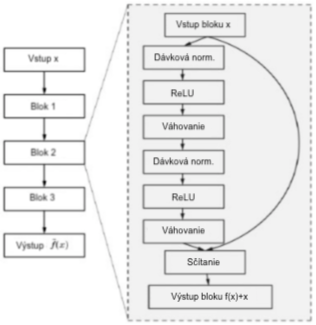
\includegraphics[width=0.4\textwidth]{images/MMD-ResNet_arch.png}}
%popis obrazku
\caption[Architektúra MMD-ResNet]{Architektúra reziduálnej siete MMD-ResNet}
%id obrazku, pomocou ktoreho sa budeme na obrazok odvolavat
\label{MMD-ResNet_arch}
\end{figure}



\section{Klasifikácia cytometrických dát}

Automatický gating je vykonávaný hlbokou doprednou neurónovou sieťou, ktorá je trénovaná na klasifikáciu buniek na základe ich parametrov. Trénovanie neurónovej siete je založené na báze učenia s učiteľom \cite{Goh1995}. Za supervíziu sú považované klasifikované bunky z  manuálne-gatovanej referenčnej vzorky. Referenčná vzorka je zvolená pred fázou trénovania neurónovej siete. 

Pre získanie referenčnej vzorky je potrebné vytvoriť $d \times d$ kovariančnú maticu pre všetky vzorky $i$, kde $d$ je počet markerov danej vzorky. Následne, pre každú permutáciu párov $i,j$ je vyrátana Forbeniova norma vzdialenosti medzi ich kovariančnými maticami ako $\left\lVert\sum_{i}-\sum_{j}\right\rVert_F$. Za referenčnú vzorku je vybraná tá vzorka, ktorá má najmenšiu priemernú vzdialenosť voči ostatným vzorkám \cite{Li2017}.

Zvolená referenčná vzorka je manuálne gatovaná. Gatovaním vzorky sa jednotlivé bunky danej vzorky zaradia (klasifikujú) do diskrétnych skupín. Bunky zaradené do diskrétnych skupín slúžia ako supervízia pre klasifikátor. Klasifikátor je trénovaný na základe manuálne gatovanej dátovej vzorky. Po absolovani trénovania je klasifikátor ďalej používaný na realizovanie automatického gatovania ďalších dátových vzoriek \cite{Li2017}.

Klasifikátor pozostáva zo skrytých vrstiev typu \textit{softplus} \cite{Goh1995} a výstupnej vrstvy typu \textit{softmax}. Veľkosť výstupnej vrstvy je závislá na počte kategórií, do ktorých sú jednotlivé bunky klasifikované (viď Obrázok \ref{cell_classifier_arch}) \cite{Li2017}.

\begin{figure}
%vlozenie samotneho obrazku vycentrovaneho a vhodnej velkosti
%obrazok je v subore images/cervik.png
\centerline{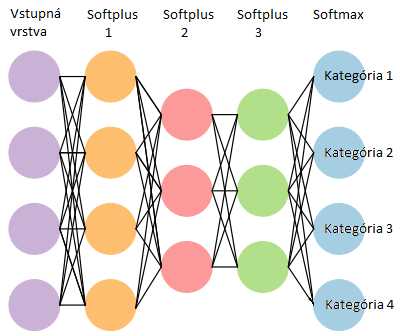
\includegraphics[width=0.4\textwidth]{images/cell_classifier_arch.png}}
%popis obrazku
\caption[Architektúra bunkového klasifikátora]{Ilustrácia architektúry neurónovej siete, ktorá klasifikuje (gatuje) jednotlivé bunky krvných vzoriek do diskrétnych skupín (kategórií) \cite{Li2017}.}
%id obrazku, pomocou ktoreho sa budeme na obrazok odvolavat
\label{cell_classifier_arch}
\end{figure}

\section{Zhrnutie analýzy cytometrických dát}

% výsledky DeepCyTOF na súťaži
Presnosť predikcií metódy DeepCyTOF je pozorovaná experimentom \cite{Li2017} a \cite{Li2016}. Experiment bol zameraný na evaluácia presnosti gatovania cytometrickej dátovej sady metódou DeepCyTOF. Podľa výsledkov experimentov, metóda DeepCyTOF presnosťou predikcií porazila výhercu súťaže FlowCAP-I. Presnosť klasifikácie buniek je na 99\% zhodná s metódou manuálneho gatovania \cite{Li2016}.

Metóda DeepCyTOF má svojou úspešnosťou veľký prínos v oblasti cytometrie, biomedicíny a lekárskej diagnostiky. Vysoká presnosť predikcií predstavuje príležitosť skorého diagnostikovania rôznych ľudských ochorení. Analýza cytometrických dát v minulosti vyžadovala veľké množstvo času, vzhľadom na náročnosť manuálneho gatovania. Využitím metódy DeepCyTOF sa naskytá príležitosť predchádzať manuálnemu gatovaniu.

Využitie reziduálnej siete na kalibráciu dátových vzoriek má svoje opodstatnenie len v prípade dátovej sady s vysokou mierou diskrepancie hodnôt jednotlivých parametrov \cite{Li2017}. Trénovaním reziduálnej siete je možné asymptoticky aproximovať identické zobrazenie (viac v \ref{residual_learning}). Využitím metriky maximálnej priemernej odchýlky je reziduálna sieť schopná aproximovať identické zobrazenia aj z rozdielnych distribúcií hodnôt. Výstupom takejto reziduálnej siete je kalibrovaná dátová vzorka, ktorá má distribúcie hodnôt parametrov príbuzné distribúciam hodnôt parametrov referenčnej vzorky. Aplikácia kalibrácie hodnôt parametrov na dátovú sadu s nízkou mierou diskrepancie môže mať nulový vplyv na výslednú presnosť predikcií metódy DeepCyTOF \cite{Li2017}.

Predmetom nášho skúmania je zistiť, aký vplyv na výslednú presnosť metódy DeepCyTOF bude mať implementácia syntetického gradientu v reziduálnej sieti vykonávajúcej kalibráciu vstupných vzoriek (MMD-ResNet).
